\chapter{STRONTIUM POLARIZABILITY MEASUREMENT PROPOSAL}
\label{alphaSrChapter}


\newcommand*{\sSz}{$^1\textrm{S}_0$~}
\newcommand*{\tPz}{$^3\textrm{P}_0$~}
\newcommand*{\tPo}{$^3\textrm{P}_1$~}
\newcommand*{\tPt}{$^3\textrm{P}_2$~}
\newcommand*{\sDt}{$^1\textrm{D}_2$~}
\newcommand*{\tDo}{$^3\textrm{D}_1$~}
\newcommand*{\sPo}{$^1\textrm{P}_1$~}
\newcommand*{\tSo}{$^3\textrm{S}_1$~}
\newcommand*{\muW}{$\mu\textrm{W}$~}

\newcommand*{\aSr}{$\alpha_\textrm{Sr}$}
\newcommand*{\aSrm}{$\alpha_\textrm{Sr*}$}


We propose to measure the strontium ground 5s$^2$ \sSz and metastable 5s5p \tPz polarizabilities to provide crucial tests of atomic structure calculations needed for next generation atomic clocks \cite{Mit10} and \cite{Lud08}. Due to uncertain polarizabilities of the clock states, the Sr and Yb clocks until recently had an uncertainty that is 70-250 times larger than their ultimate lifetime-limited precision \cite{Lud08, Lem09}. The polarizability influences the clock frequency because blackbody radiation from the thermal environment causes relatively large, uncertain Stark shifts of the clock states. Recent \emph{in situ} measurements of the differential polarizability of the clock states of Sr \cite{Mid12a} and Yb \cite{She12} have significantly reduced the uncertainties due to the BBR shift. However, measurements of the polarizabilities of the individual states are still in high demand due to the importance of accurate calibration of the BBR shift and due to the difficulty of calculating these polarizabilities.

In this chapter we will discuss in detail the three technical challenges of measuring \aSr~ and \aSrm:
\begin{itemize}
\item Detection of ground state Sr with resonant photoionization. 
\item Detection of metastable state Sr using resonant and non-resonant photoionization.
\item Metastable Sr generation using electron impact ionization.
\end{itemize}




\begin{figure}
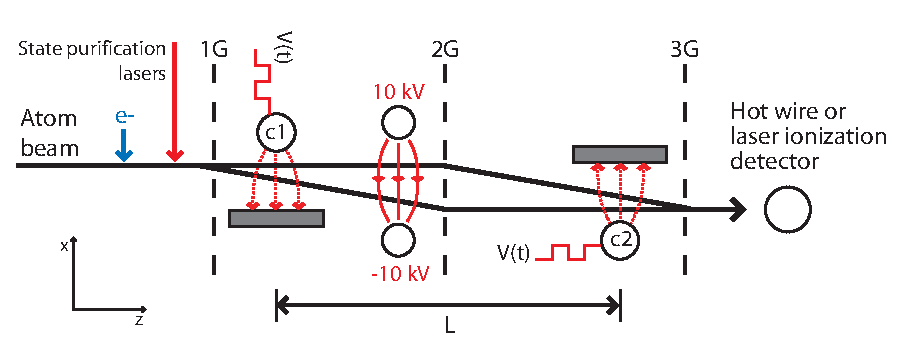
\includegraphics[width=1\textwidth]{Figures/IFMgradEfigNIST2011full.eps}
\caption[Atom interferometer configuration for strontium and ytterbium polarizability measurements.]{\label{IFMgradEfigSrYb}Atom interferometer set-up for strontium and ytterbium polarizability measurements. Nanogratings 1G, 2G, and 3G form a Mach-Zehnder atom interferometer. To measure beam velocity, we apply a periodic voltage $V(t)$ to two phase choppers (c1 and c2) separated by a distance $L$ and study the contrast of the interferometer as a function of switching frequency. To measure polarizability, we apply $\pm10$ kV across the interferometer to induce a polarizability-dependent phase shift. We will use an electron bombardment region to promote Sr and Yb atoms to a metastable state, followed by resonant lasers to purify the beam in the $^3\textrm{P}_0$ state. Beam detection will be accomplished with resonant laser ionization. Diagram not to scale.}
\end{figure}





%%%%%%%%%%%%%%%%%%%%%%%
\section{Detection of ground state Sr}

%%%%%
\subsection{Photoionization via 461 and 405 nm transitions}
The ionization energy of the ground 5s$^2$ \sSz state of strontium is 5.7 eV. This high ionization energy makes strontium difficult to ionize using our current hot-wire detector. We will discuss an efficient resonant photoionization pathway via a 461 nm photon to the 5s5p \sPo state and a 405 nm photon to the autoionizing state 5p$^2$ \sDt \cite{Men95,Van06,Haq07} (see Figure \ref{SrTerm}). We show that resonant photoionization will provide $\sim$20\% ionization probability with nearly zero background. We will assume that all lasers will be focused to a spot size of $A$=(100 $\mu\textrm{m})^2$ and that the atom beam velocity $v=3000$ m/s.

The \sSz- \sPo transition at 461 nm has an $A_{21}$ coefficient of $1.9\times10^8$ Hz. This corresponds to a state lifetime $\tau=5.3$ ns and $I_\textrm{sat}= 40$ mW/cm$^2$. Assuming a spot size of (100 $\mu\textrm{m})^2 =10^{-8}\textrm{ m}^2$, 4 $\mu\textrm{W}$ is needed to saturate this transition. The Rabi frequency $\Omega = \Gamma \sqrt{I/2I_{sat}}$ and for a two-state atom $\Gamma=A_{21}$. We will approximate the probability of finding a two-level atom in the excited state when $I=I_\textrm{sat}$ as $P\approx1/2$.


\begin{figure}
\centerline{\includegraphics[scale=0.65]{Figures/LudlowSrDiagramMod.pdf}}
\caption[Strontium term diagram.]{\label{SrTerm}Sr term diagram. Transition wavelengths (nm), photon energies (eV), Einstein $A_{21}$ coefficients (Hz), lifetimes (ns), and $I_\textrm{sat}$ (mW/cm$^2$) are shown next to each transition. Adapted from Ludlow \cite{Lud08}. Note: $\Omega = \Gamma \sqrt{2I/I_{sat}}$.}
\end{figure}


Absorption of a 405 nm photon takes an atom in the excited 5s5p \sPo to the 5p$^2$ \sDt autoionizing state. The presence of this autoionizing state causes the ionization cross-section of the \sPo state with 405 nm light to be $10^3$ to $10^6$ times larger than typical non-resonant photoionization cross-sections: $\sigma=5600$ Mb (1 Mb = $10^{-22}$ m$^2$). 


We will now calculate the ionization probability a strontium atom in the ground state via this resonant ionization path. First, we write the single atom ionization rate from the \sPo state as 
\begin{eqnarray}
\Gamma_{1\textrm{P}1-\textrm{Sr}^+} = \sigma\Phi_\gamma = \sigma \frac{I_{405}}{E_\gamma} 
\end{eqnarray}
where $\sigma$ is the ionization cross-section, $\Phi_\gamma$ is the 405 nm photon flux, $I_{405}$ is the laser intensity for a beam with power $P_{405}$ focused to a spot size $A$, and $E_\gamma=hc/\lambda$ is the photon energy. We calculate $\Gamma_{1\textrm{P}1-\textrm{Sr}^+} = 10^7$ s$^{-1}$, assuming $P_{405}=100$ mW and A=(100 $\mu\textrm{m})^2$. Next, we must consider the time that the atom beam interacts with the ionization laser: $T=l/v$, where $l=\sqrt{A}$ is the interaction length. $T=30$ ns, assuming a beam velocity of 3000 m/s. The probability of photoionization from the \sPo state is then
\begin{eqnarray}
\textrm{Prob}_{1\textrm{P}1-\textrm{Sr}^+} = \Gamma_{1\textrm{P}1-\textrm{Sr}^+} T = \sigma \frac{P}{E_\gamma v \sqrt{A}}.
\end{eqnarray}
Using the above assumptions, we calculate an ionization probability of 38\% from the \sPo state. We assume that the intensity of light resonant with the \sSz - \sPo transition is sufficient to put atoms in the \sPo state 50\% of the time, and then estimate the ground state ionization probability of our system to be $\textrm{Prob}_{1\textrm{S}0-\textrm{Sr}^+}=10-20\%$. 


This resonant photoionization detection efficiency is comparable to our hot-wire detector efficiency with potassium, rubidium, and cesium atoms. However, the resonant photoionization method will presumably have a much lower noise floor than the hot-wire method. Therefore, we can expect that resonant photoionization will work for our system even if our ionization probability estimates are off by several orders of magnitude.



%%%%%%
\subsection{Generating 461 and 405 nm light}
Several possibilities exist for generating 461 nm light: frequency doubling 922 nm light, a blue LED, a strontium hollow cathode lamp, and an AR-coated laser diode.


First, we discuss second harmonic generation of 461 nm light. The efficiency of SHG of 922 nm to 461 nm varies from 0.01-75\% \cite{Van06,Tar05} depending on the effort expended, expertise of the lab, cavity specifications, and type of crystal used. A PPKTP crystal can achieve 1\% conversion efficiency with a single pass through the crystal when pumped with about 100 mW of 992 nm light, so no cavity would be needed. This may yield sufficient power and would be relatively simple. The crystal would need to be temperature tuned to 40-70 $^\circ$C. We estimate that it is reasonable that 100 \muW of resonant 461 nm light may delivered to the beam using SHG with a PPKTP. A prototype in our lab using a PPKTP crystal currently outputs about 10 \muW of 461 nm light.


We also explored several other methods to generate 461 nm light. Blue LEDs with center wavelengths near 460 nm provide another possibility for generating 461 nm light. LEDs with optical powers of 1 W are available. The typical $\Delta\lambda=25$ nm, corresponding to a frequency dispersion of $df=c/\lambda^2d\lambda=3\times10^{13}$ Hz. The linewidth of the \sSz-\sPo transition is 30 MHz, so approximately $10^{-6}$ of the light generated in the LED, 0.1-1 $\mu$W, may be resonant with the atom beam. 


Hollow cathode lamps are typically specified as producing 10-20 mA discharge current, however, the corresponding optical power is unknown. Typical operating voltages are 300 V. We assume an optical output power $P$, and that owing to the extended nature of the source, only 10\% of the light may be delivered to the atom beam. The doppler-broadening of the light from a hollow cathode lamp will further reduce the effective power. We assume a temperature of 900 K and calculate a corresponding doppler width of 1.5 GHz. The linewidth of the \sSz-\sPo transition is 30 MHz, so approximately 2\% of the light generated in the lamp may be resonant with the atom beam. The above factors yield an efficiency of $0.002P$. Hollow cathode lamps are relatively inexpensive (\$355), and require a 550 V, 20 mA power supply (available for \$2125, although we have a supply that would probably work). Hollow cathode lamp lifetimes are warranted to 5000 mA hours. At 10 mA, the lifetime would be 500 hours, or about 20 days of continuous operation. This can be quickly implemented with little expertise, and may provide sufficient power. 


Finally, Shimada \etal recently used a prototype AR coated diode from Nichia to generate 40 mW at 461 nm from an ECDL \cite{Shi13}. Commercialization of this diode technology would greatly simplify our strontium polarizability measurement.





%%%%%%%%%%%%%%%%%%%%%%%
\section{Detection of metastable Sr}


We now consider photoionization of the metastable \tPz state. To our knowledge, no autoionizing triplet states exist, so non-resonant photoionization must be used with the metastable state. The ionization energy of the \tPz state is 3.9 eV (318 nm). Therefore, direct photoionization of the \tPz state would require an intense UV source. The near-threshold photoionization cross-section of the \tPo state is $\sigma_{3P1}\approx 10$ Mb \cite{Haq07}. A UV lamp may provide sufficient power at this wavelength to directly ionize the \tPz state. Wang \cite{Wan11} used a UV LED to photoionize \tPz Ba atoms. We are exploring if we can use UV light to photoionize the \tPz with sufficient efficiency. UV LEDs with 0.5 mW available for $\sim$\$150. High power (0.5 W) UV LEDs are common down to 365 nm.

We also considered the possibility of using a two photon ionization process via the 5s5p \tPz to 5s6s \tSo at 679 nm (1.8 eV), and then an ionizing photon with $\lambda<590$ nm (2.1 eV). To our knowledge, no published photoionization cross-sections exist for the 5s6s \tSo state. Therefore, we estimate that the photoionization cross-section for the \tSo state is similar to that of the 5s6s \sSz state: $\sigma_{1S0}=0.4$ Mb \cite{Sam06}. \tSo will also decay to \tPo and \tPt, so we must apply the state purification lasers at detector as well to keep atoms in the \tSo state.

Another possible intermediate state is 5p$^2$ $^3\textrm{P}_1$. The transition between 5s5p \tPz and 5p$^2$ \tPo is at 474 nm (2.6 eV). The transition rate is $4\times10^7$ Hz \cite{Por08}. A photon with $\lambda< 950$ nm (1.31 eV) would be needed to photoionize the 5p$^2$ \tPo state. 473 nm diodes with several 10s of mW are available from several sources, including ThorLabs.

Yet another possible intermediate state is 5s5d \tDo. The transition between 5s5p \tPz and 5s5d \tDo is at 483 nm (2.6 eV). The transition rate is $4\times10^7$ Hz \cite{Por08}. A photon with $\lambda< 915$ nm (1.35 eV) would be needed to photoionize the 5s5d \tDo state. 490 nm diodes with several 10s of mW are available from several sources (Renesas NX6414EH, CrystaLaser, ThorLabs).




\section{Generating metastable Sr}

Metastable strontium and ytterbium will be generated in an electron bombardment region \cite{Giu88} and state purification will be accomplished with resonant lasers. The electron bombardment region will populate the nsnp$^3$P metastable triplets with 40\% efficiency. We will build diode lasers at 679 and 707 nm to optically pump metastable strontium atoms from the $^3\textrm{P}_1$ and $^3\textrm{P}_2$ states into the $^3\textrm{P}_0$ state. We will also build diode lasers at 649 and 770 nm to purify the ytterbium metastable triplet. We have prototypes of two of these lasers (679 and 770 nm) available from experiments with lithium and potassium atoms.




